\documentclass{beamer}


% ---
% PACOTES
% ---

% ---
% Pacotes fundamentais 
% ---
\usepackage{times}         % Usa a fonte Latin Modern
\usepackage[T1]{fontenc}      % Selecao de codigos de fonte.
\usepackage[utf8]{inputenc}      % Codificacao do documento (conversão automática dos acentos)
\usepackage{indentfirst}      % Indenta o primeiro parágrafo de cada seção.
\usepackage{nomencl}          % Lista de simbolos
\usepackage{color}            % Controle das cores
\usepackage{graphicx}         % Inclusão de gráficos
\usepackage{microtype}        % para melhorias de justificação
\usepackage{ordinalpt}
% ---
% ---
% Pacotes adicionais, usados apenas no âmbito do Modelo Canônico do abnteX2
% ---
\usepackage{lipsum}           % para geração de dummy text
% ---
      
% ---
% Pacotes de citações
% ---
\usepackage[brazilian,hyperpageref]{backref}  % Paginas com as citações na bibl
\usepackage[alf]{abntex2cite} % Citações padrão ABNT
% ---


\usetheme{Warsaw}
\usecolortheme{wolverine}

% ---
% Configurações do pacote backref
% Usado sem a opção hyperpageref de backref
\renewcommand{\backrefpagesname}{Citado na(s) página(s):~}
% Texto padrão antes do número das páginas
\renewcommand{\backref}{}
% Define os textos da citação
\renewcommand*{\backrefalt}[4]{
   \ifcase #1 %
      Nenhuma citação no texto.%
   \or
      Citado na página #2.%
   \else
      Citado #1 vezes nas páginas #2.%
   \fi}%
% ---
\usetheme{Berlin}

% --- Informações de dados para CAPA e FOLHA DE ROSTO ---
\title{Representações sociais da poluição nas práticas de ensino: \\
Estado do conhecimento}

\author{João Henrique da Silva\\
--
Prof. Dr. Carlos Alberto de Oliveira Magalhães Júnior}
\institute{UEM DCI PROFCIAMB}
\logo{

\includegraphics[width=1cm]{logo.png}

\includegraphics[width=1cm]{uem.png}
}

%\local{Brasil}
\date{Dezembro - 2022}
% ---

% ---
% Configurações de aparência do PDF final

% alterando o aspecto da cor azul
\definecolor{blue}{RGB}{41,5,195}

% informações do PDF
\makeatletter
\hypersetup{
      %pagebackref=true,
      pdftitle={\@title}, 
      pdfauthor={\@author},
      pdfsubject={},
      pdfcreator={},
      pdfkeywords={abnt}{latex}{abntex}{abntex2}{atigo científico}, 
      colorlinks=true,           % false: boxed links; true: colored links
      linkcolor=blue,            % color of internal links
      citecolor=blue,            % color of links to bibliography
      filecolor=magenta,            % color of file links
      urlcolor=blue,
      bookmarksdepth=4
}
\makeatother
% --- 

% ---
% compila o indice
% ---
\makeindex
% ---



% --- 
% Espaçamentos entre linhas e parágrafos 
% --- 

% O tamanho do parágrafo é dado por:
\setlength{\parindent}{1.3cm}

% Controle do espaçamento entre um parágrafo e outro:
\setlength{\parskip}{0.2cm}  % tente também \onelineskip

% Espaçamento simples
\linespread{1.3}


%\usetheme{lucid}
\begin{document}
    \frame {
        \titlepage
    }

    \frame {
        \frametitle{Representações sociais - RS}
        \framesubtitle{A contribuição de \citeonline{Representacees_sociais_moscovici}}
	\begin{itemize}
		\item A análise qualitativa de conteúdos requer ferramentas heurísticas, como a metodologia das representações sociais.
		\item Metodologia presente em textos monográficos, teses de doutorado e dissertações de mestrados presentes no catálogo de Teses e Dissertações da \citeonline{catalogo_capes}.
        \item Metodologia quanti-quali, análise da produção acadêmica : quantitativa seguida de qualitativa \cite{Python_NLTK_capes}.

	\end{itemize}
    }

    \frame{
        \frametitle{Resultados e discussões}
        \framesubtitle{Representações sociais no ano de 2021 - 01}
        \begin{figure}
          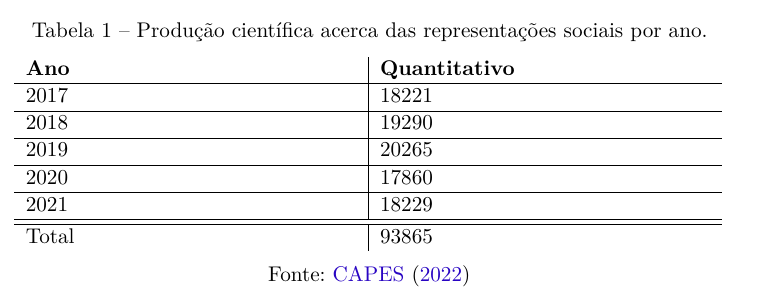
\includegraphics[width=80mm,scale=1]{tab_01.png}
        \end{figure}
    }

    \frame{
        \frametitle{Resultados e discussões}
        \framesubtitle{Modalidades da produção no ano de 2021 - 02}
        \begin{figure}
          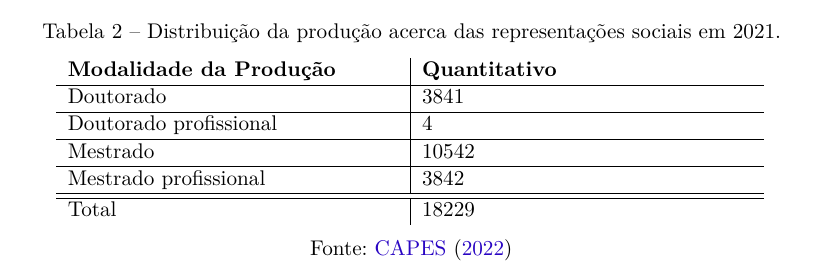
\includegraphics[width=80mm,scale=1]{tab_02.png}
        \end{figure}
    }

    \frame{
        \frametitle{Resultados e discussões}
        \framesubtitle{Modalidades da produção no ano de 2021 - 03}
        \begin{figure}
            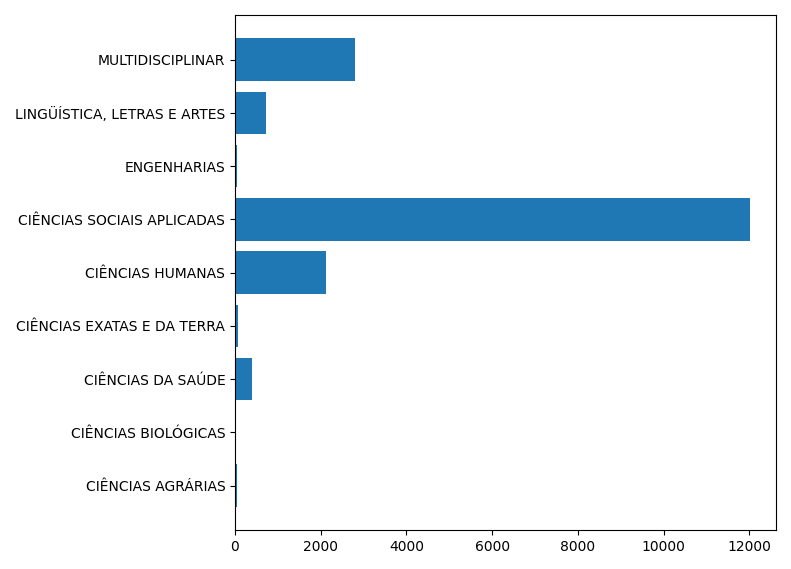
\includegraphics[width=80mm,scale=1]{est_con_2021.png}
        \end{figure}
    }

    \frame{
        \frametitle{Análise quantitativa - 01}
        \begin{itemize}
            \item O quantitativo de resultados retornado pelo referido banco de dados ao se expandir o escopo da pesquisa proposta para contemplar os quatro seguintes termos-chave 'representações sociais ensino ensino ambiental' surpreende pela abrangência, ao totalizar 480821 publicações.
            \item Possíveis viéses no mecanismo de busca da Capes?
        \end{itemize}
    }

    \frame{
        \frametitle{Análise qualitativa - 02}
        \begin{itemize}
            \item Dentro dos resumos das 105 publicações selecionadas, encontra-se a terminologia que interessa à pesquisa proposta ao se identificar a ocorrência e coocorrência de quatro termos específicos, sendo estes, em ordem de prioridade: 'representações', 'sociais', 'ensino' e 'poluição', os quais foram identificados no material selecionado através da busca por seus respectivos elementos radicais, i.e. 'represent', 'soc', 'ensin' e 'polu'.
            \item Seleções de grupos de textos para leitura.

        \end{itemize}
    }

   

    \frame{
        \frametitle{Análise qualitativa - 03 - Meta 9.1}
        \begin{itemize}
            \item Nações Unidas Desenvolver infraestrutura de qualidade, confiável, sustentável e resiliente, incluindo infraestrutura regional e transfronteiriça, para apoiar o desenvolvimento econômico e o bem-estar humano, com foco no acesso equitativo e a preços acessíveis para todos. \citeonline{Agenda_2030}
            \item Construir infraestrutura resiliente, promover a industrialização inclusiva e sustentável, e fomentar a inovação
            \item Atende ao ODS 9 - Construir infraestrutura resiliente, promover a industrialização inclusiva e sustentável, e fomentar a inovação
        \end{itemize}
    }


    \frame{
        \frametitle{Análise qualitativa - 04 - Meta 9.c}
        \begin{itemize}
            \item Nações Unidas Aumentar significativamente o acesso às tecnologias de informação e comunicação e empenhar-se para procurar ao máximo oferecer acesso universal e a preços acessíveis à internet nos países menos desenvolvidos, até 2020.
            \item Brasil Aumentar significativamente o acesso às tecnologias de informação e comunicação e empenhar-se para oferecer acesso universal e a preços acessíveis à internet, até 2020, buscando garantir a qualidade, a privacidade, a proteção de dados e a segurança cibernética.
        \end{itemize}
    }


    \frame{
        \frametitle{Diagrama de Reinert}
        \begin{figure}
            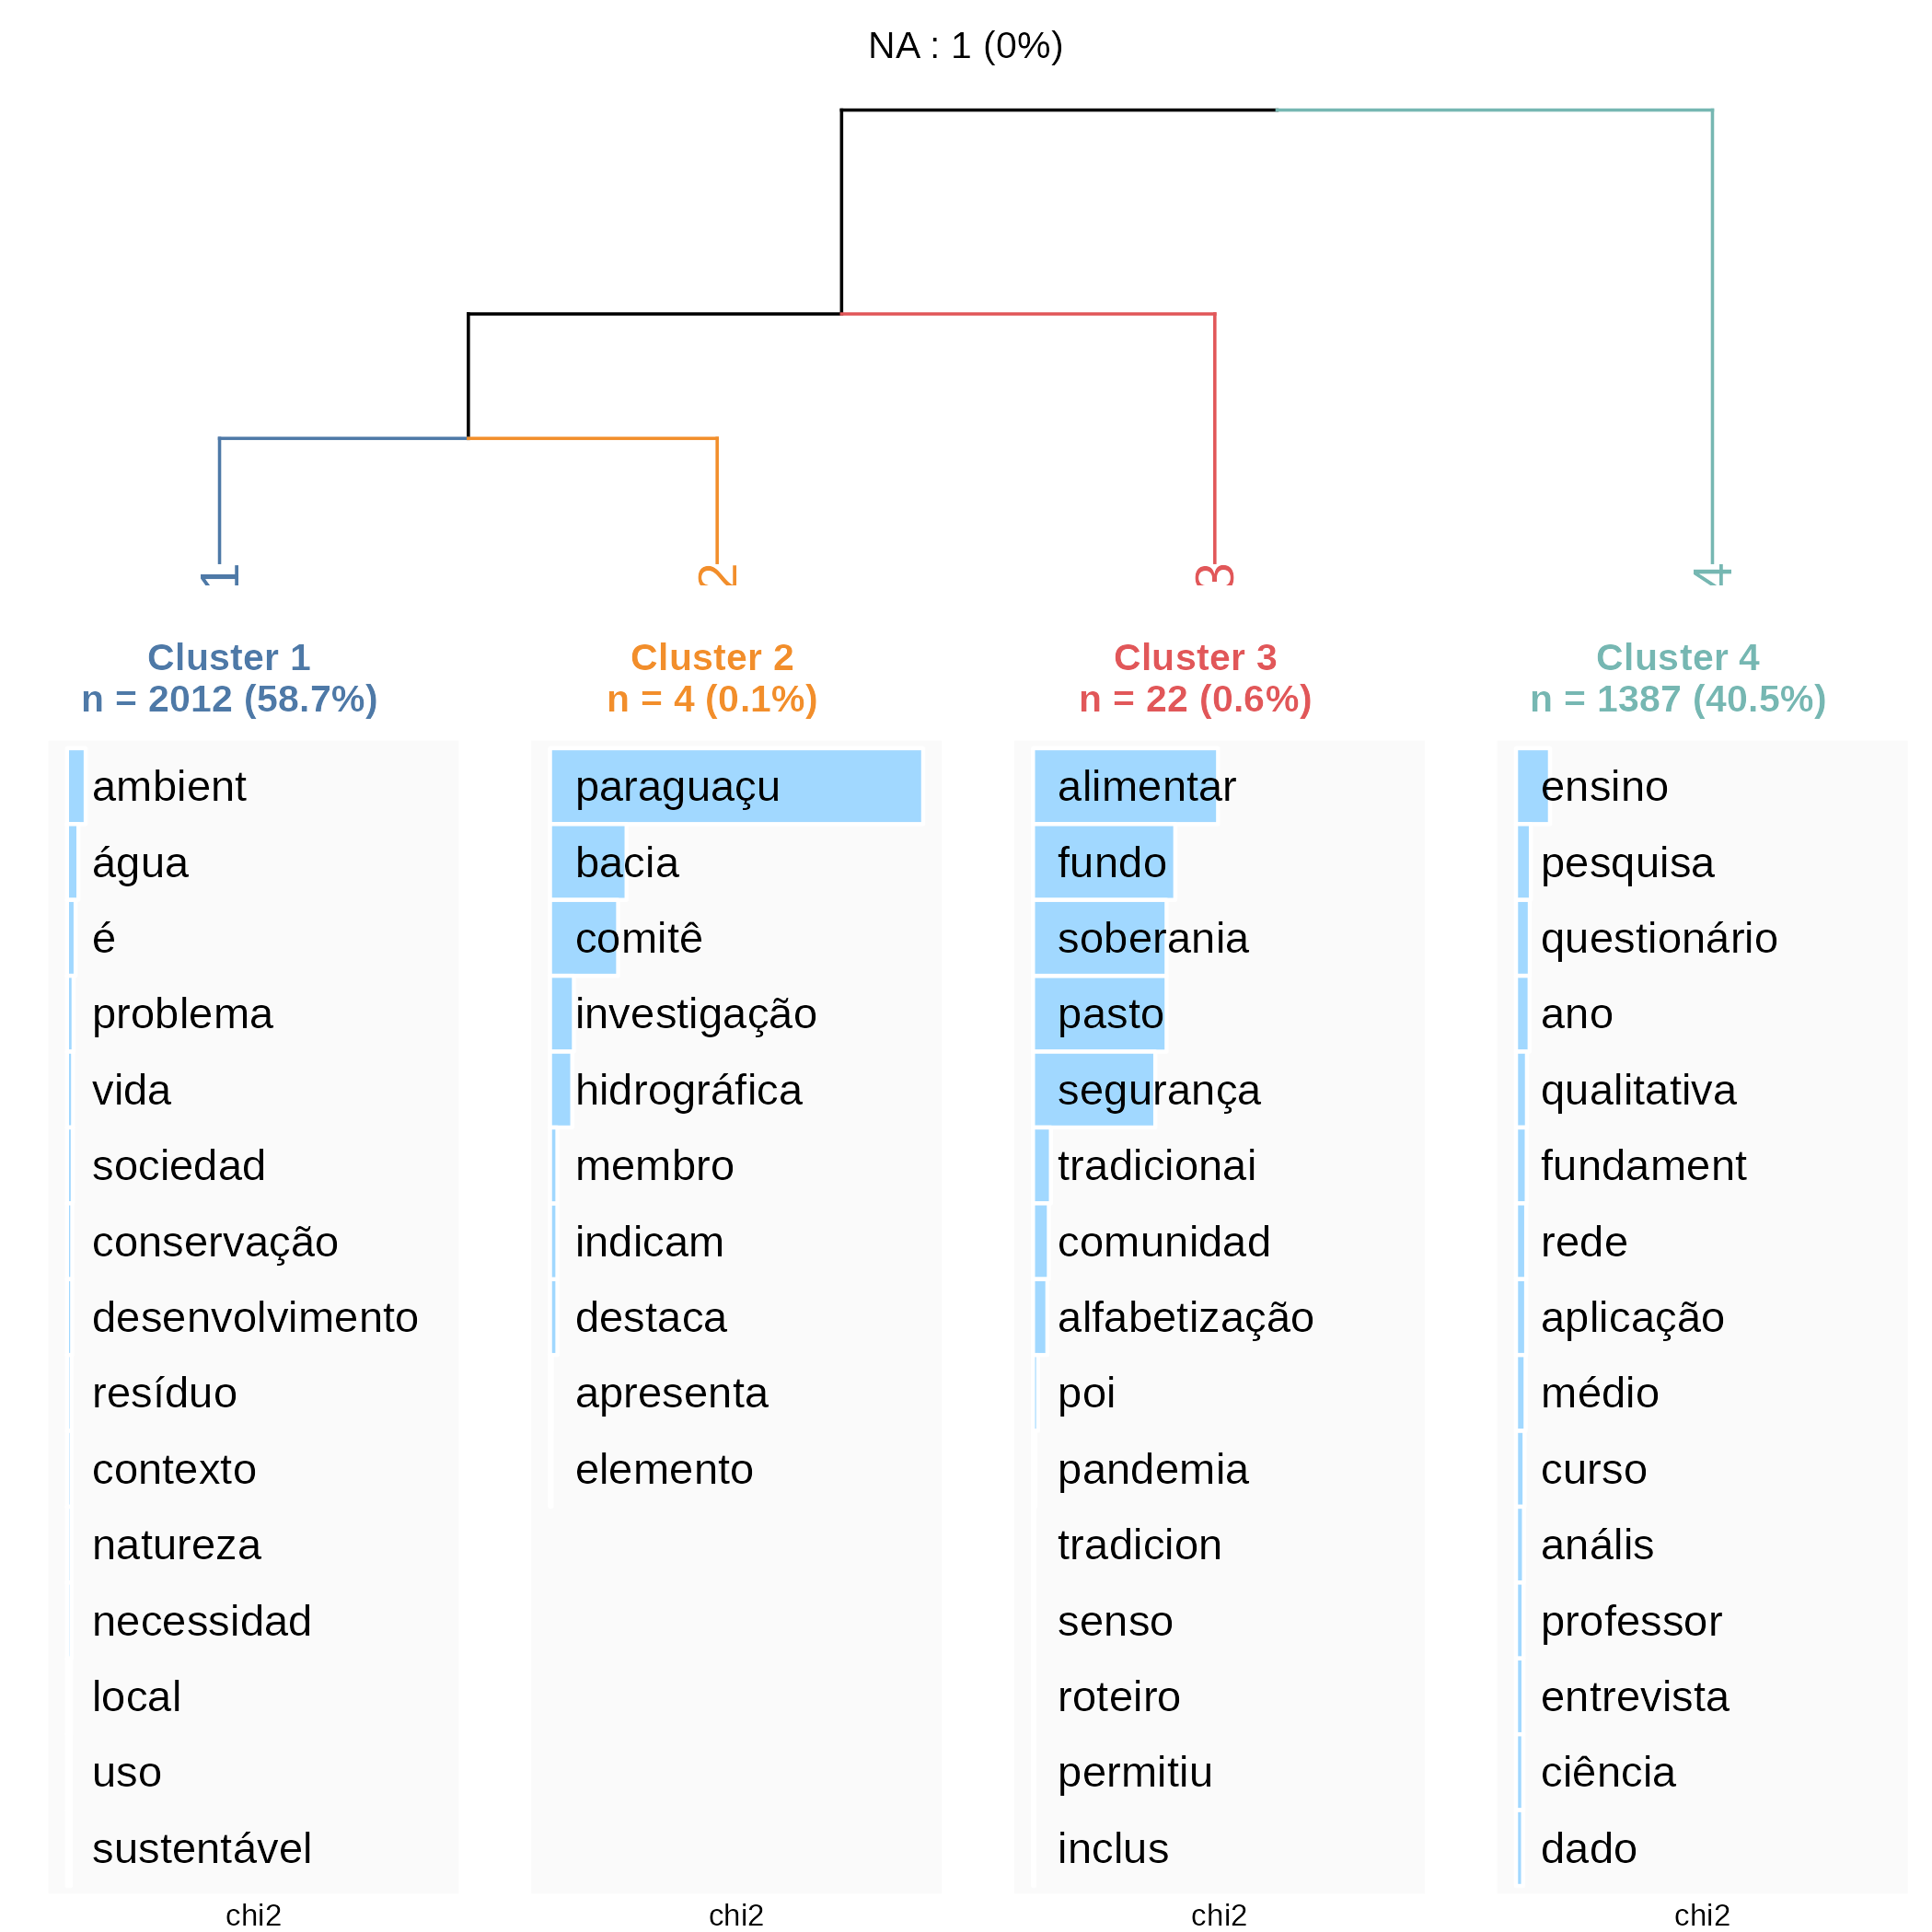
\includegraphics[width=80mm,scale=0.8]{resumes_reinert.png}
        \end{figure}
    }

    \frame{
        \frametitle{Representações e ensino}
        \begin{itemize}
            \item {O termo representações aparece isolado nos resumos em apenas 9 das publicações selecionadas; percebe-se daí que a presença do termo, verificada usando o radical, coocorre junto ao termo ensino e se apresenta em 15 trabalhos, dentro dos selecionados. Quando se soma aos termos 'representações' e 'ensino', a terceira categoria 'sociais' afim de denotar a convergência proposta pelo recorte adotado, a quantidade de trabalhos cujos resumos carregam tais temas se expande para 19 obras.}
        \end{itemize}

    }
    
    \frame{
        \frametitle{Representações da poluição segundo discentes do ensino fundamental}
        \begin{itemize}
            \item {O recorte pode ser expandido para incluir outros elementos relevantes. Ao se considerar a coocorrência do termo fundamental, denotado pelo radical 'fundament', expande-se o escopo dos trabalhos e encontra-se 29 obras cujos resumos carregam tais temas. Ao se incluir o objeto 'poluição' denotado pelo radical 'polu', a quantidade de trabalhos cujos resumos carregam tais temas se expande para 34 obras.}
        \end{itemize}
    }
    
    \frame{
        \frametitle{Representações segundo discentes do Novo Ensino Médio}
        \begin{itemize}
            \item {O tema do Novo Ensino Médio, não foi encontrado nos resumos selecionados, situação que indica a necessidade de se realizarem estudos originais, dentro deste recorte da educação contemporânea.}
        \end{itemize}
    }
    
    \frame{
        \frametitle{Representações da poluição e geração de energia}
        \begin{itemize}
            \item {Ao se expandir o tema e incorporar outros elementos, percebe-se que o escopo das obras ilustra a capilaridade e o caráter interdisciplinar das investigações. O termo energia, denotado pelo radical 'energ' coocorre com os termos 'representações', 'ensino', 'poluição' gerando um conjunto de 26 obras cujos resumos abordam tais objetos.}
        \end{itemize}
    }

    \frame{
        \frametitle{Representações da poluição, consumo e lixo}
        \begin{itemize}
            \item {O agregado mais amplo apresentado aqui incorpora os termos acima apresentados e soma os termos 'fundamental' 'indústria' e 'lixo', denotados pelos respectivos radicais 'fundament', 'indústr', 'lix', gerando um conjunto de 52 obras cujos resumos apresentam tais termos.}
        \end{itemize}
    }

    \frame{
        \frametitle{Considerações finais - 01}
        \begin{itemize}
            \item {Percebe-se que o escopo da terminologia usada nas palavras-chave da pesquisa proposta permeia diversas áreas do conhecimento. Destaca-se aí o caráter interdisciplinar das propostas em educação ambiental, característica que exigem a filtragem dos resultados apresentados pelo referido portal. A seleção de obras no banco de dados da Capes deve ser então seguida de um processo de filtragem similar ao processo aqui apresentado, o qual permita perceber e selecionar grupos de obras as quais compartilhem temas e métodos. }
        \end{itemize}
    }

    \frame{
        \frametitle{Considerações finais - 02}
        \begin{itemize}
            \item {Acerca especificamente do tema das representações sociais, este se apresenta difundido em diversas áreas do conhecimento, com especial destaque para as áreas de ciências sociais aplicadas, multidisciplinar, e da linguística. A aplicação de tal metodologia nos estudos da educação está contemplada, de maneira implícita, nestes três recortes. A ausência de estudos de estudos de representações sociais no contexto do Novo Ensino Médio é um fato de destaque, dado pela novidade do formato de ensino em questão.}
        \end{itemize}
    }   
\bibliography{interdisciplinaridade}
\end{document}



